\subsection*{Teil D: Grafische Darstellungen interpretieren (5 Minuten)}

\begin{enumerate}[label=\arabic*.,resume]

    \item \textbf{Diagramm interpretieren:}

    Der Graph zeigt die Fahrt eines Autos:

    \begin{center}
        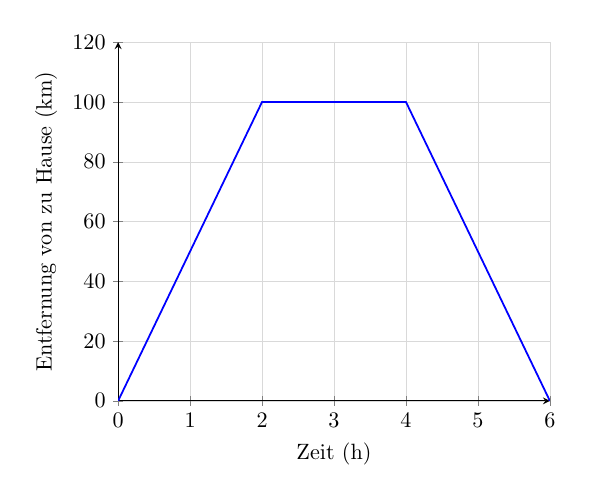
\begin{tikzpicture}[scale=0.8]
            \begin{axis}[
                axis lines = left,
                xlabel = {Zeit (h)},
                ylabel = {Entfernung von zu Hause (km)},
                xmin=0, xmax=6,
                ymin=0, ymax=120,
                xtick={0,1,2,3,4,5,6},
                ytick={0,20,40,60,80,100,120},
                grid=major,
                grid style={line width=0.1pt,draw=gray!30},
            ]
            \addplot[thick, blue] coordinates {(0,0) (2,100) (4,100) (6,0)};
            \end{axis}
        \end{tikzpicture}
    \end{center}

    \begin{enumerate}[label=\alph*)]
        \item Wie weit ist das Auto nach 2 Stunden von zu Hause entfernt? \underline{\hspace{3cm}}

        \item Was passiert zwischen der 2. und 4. Stunde? \underline{\hspace{6cm}}

        \item Wie lange dauert die Rückfahrt? \underline{\hspace{4cm}}
    \end{enumerate}

\end{enumerate}